\documentclass{article}%
\usepackage[T1]{fontenc}%
\usepackage[utf8]{inputenc}%
\usepackage{lmodern}%
\usepackage{textcomp}%
\usepackage{lastpage}%
\usepackage{authblk}%
\usepackage{graphicx}%
%
\title{The Retromer Complex Is Required for Rhodopsin Recycling and Its Loss Leads to Photoreceptor Degeneration}%
\author{Sean Castro}%
\affil{School of Dentistry, Chung Shan Medical University, Taichung 40201, Taiwan}%
\date{01{-}01{-}2006}%
%
\begin{document}%
\normalsize%
\maketitle%
\section{Abstract}%
\label{sec:Abstract}%
To receive an email each time a new Portola Valley News story is published, click here.\newline%
News:\newline%
Staff:\newline%
11:15 AM | Level 12\newline%
Jessica Salatin is a Assistant Editor for the Portola Valley News.\newline%
See all her blogs on Think Local.\newline%
To receive her columns sent by e{-}mail, visit JessicaSalatin.blogspot.com.\newline%
Personal Diaries\newline%
Thinking About the Environment\newline%
Don Durands Wildlife Photographer of the Year 2001\newline%
This series explores the strange, rich history of Portola Valleys flora and fauna.\newline%
Portola Valley News Newsletter\newline%
This week: Portola Valley High School spring quarter begins.\newline%
Overview and Statistics\newline%
Receiving their honors from the CRSAC National Science Fair, Portola Valley High School students Merrin Shappell and Amy Scott moved on to represent the United States in the international competition sponsored by NASA. The Science Fair is one of the largest science programs in the country. Each year, more than 130 college students from 27 countries compete to win the special awards.\newline%
An array of medals, awards and plaques are displayed on the library floor at the University of California{-}Monterey Bay Palliative Care Center. The hospital has been awarded multiple fellowships. Most recently, the institution received the Center for Palliative Care Agency of Excellence Award for Excellence in Teaching.\newline%
The undergraduate school will hold its semiannual awards ceremony for nominations for the U.S. Department of Educations Student Trust Fund that are put up for awards. Students who have had the best degree research awarded as a result of their efforts can obtain an award certificate upon the presentation of their degree. At least three students will be awarded the investment award of up to \$500.\newline%
Correction: The story in this blog was posted Tuesday, January 1, 2006 at 1:07 pm. The following post has been amended. An earlier version mistakenly listed Los Angeles College as among the top colleges to receive awards. The post has been updated accordingly.

%
\subsection{Image Analysis}%
\label{subsec:ImageAnalysis}%


\begin{figure}[h!]%
\centering%
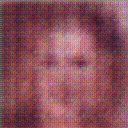
\includegraphics[width=150px]{500_fake_images/samples_5_179.png}%
\caption{A Black And White Photo Of A Small Room}%
\end{figure}

%
\end{document}